\documentclass[compress,12pt]{beamer}

\usepackage{url}
\usepackage{booktabs}

% This theme has a fairly comprehensive navigation bar at the top,
% you don't really need to periodically show the table of contents
% because it is always visible at the top.
\usetheme{Darmstadt}
\usecolortheme{sidebartab} 
\setbeamercovered{invisible}

\newcommand{\bv}[1]{{\boldsymbol{#1}}}
\newcommand{\dgammadT}{\frac{\partial \gamma}{\partial T}}
\newcommand{\Benard}{B$\acute{\text{e}}$nard}

\title{Parallel Computing on Beowulf Clusters: Performance and Applications}
\author{
  John W.\ Peterson\inst{1}
  \and
  Dr.\ Graham F.\ Carey\inst{1}
  \and
  Dr.\ William L.\ Barth\inst{2}
  \and
  Benjamin S.\ Kirk\inst{1,3}
  \and
  Dr.\ Saeed Iqbal\inst{4}
}

\institute{
\inst{1}CFDLab, The University of Texas at Austin
\and
\inst{2}Texas Advanced Computing Center (TACC)
\and
\inst{3}NASA/JSC, Applied Aerosciences \& CFD Branch
\and
\inst{4}Dell Corporation
}

\date{July 15, 2004}


% \MyLogo{SIAM 2004 Annual Meeting, Portland}
% \rightheader{\includegraphics[height=.7in]{figures/word3}}
% \leftheader{\includegraphics[height=.7in]{figures/utlogo}}

\begin{document}

\begin{frame}
  \titlepage
\end{frame}



%%%%%%%%%%%%%%%%%%%%%%%%%%%%%%%%%%%%%%%%%%%%%%%%%%%%%%%%%%%%%%%%%%%%%%%%%%%%%%%

% Not necessary with Darmstadt
% \begin{frame}
% \tableofcontents[hideallsubsections]
% \end{frame}




\section{Introduction}

%%%%%%%%%%%%%%%%%%%%%%%%%%%%%%%%%%%%%%%%%%%%%%%%%%%%%%%%%%%%%%%%%%%%%%%%%%%%%%%
\begin{frame}%{Introduction}
 \begin{minipage}[h]{.4\textwidth}
   \textbf{A general class of time-dependent nonlinear elliptic PDEs:}
   find $u(\bv{x},t)$ such that
   \begin{eqnarray}
     \label{eqn:general_pde}
     \nonumber
     \frac{\partial u}{\partial t} + \mathcal{N}( u ) & = & 0 \;\;\;\;\; \in \Omega \\
     \nonumber
   u & = & u_D \;\; \in \partial \Omega_D \\
   \nonumber
   \nabla u \cdot \bv{n} & = & u_N \;\; \in \partial \Omega_N \\
   \nonumber
   u(\bv{x}, 0) & = & u_0(\bv{x}) 
   \end{eqnarray}
 \end{minipage}
 \hspace{0.5in}
 \begin{minipage}[h]{.4\textwidth}
   \includegraphics[width=\textwidth]{figures/domain}
 \end{minipage}

\vspace{.05\textheight}

 \begin{itemize}
   \item $\mathcal{N}( u )$ is a nonlinear operator which depends on the unknown
     $u$ and its spatial gradients%, $\bv{f}$ is a forcing function
   % \item With slight modifications, a wide range of physically interesting problems fall into this class
   \item Use generic numerical methods to treat many problems in the same framework
 \end{itemize}
\end{frame}



%%%%%%%%%%%%%%%%%%%%%%%%%%%%%%%%%%%%%%%%%%%%%%%%%%%%%%%%%%%%%%%%%%%%%%%%%%%%%%%
\begin{frame}%{Introduction}
   \begin{itemize}
     \item Time discretization is via finite differences ($\theta$-method)
       \begin{equation}
	 \label{eqn:theta}
	 \nonumber
	 %% 	 u^{n+1} = u^n + \Delta t \Big[ \theta \mathcal{N}( u^{n+1} )
	 %% 	 + (1-\theta)\mathcal{N}( u^{n} )\Big]
	 G(u) := u^{n+1} - u^n - \Delta t \Big[ \theta \mathcal{N}( u^{n+1} )
 	   + (1-\theta)\mathcal{N}( u^{n} )\Big] = 0
       \end{equation}
     \item Spatial discretization by Galerkin finite element method ($u \approx u_h$)
       \begin{equation}
	 \label{eqn:galerkin}
	 \nonumber
	 F(u) := <G(u_h), v_h> = 0 \;\;\; \forall \; v_h
       \end{equation}
     \item Linearization with Newton's Method
       \begin{equation}
	 \nonumber
	 F(u_{k+1}) \approx F(u_{k}) +
	 \frac{\partial F}{\partial u}\Big|_{u_k} (u_{k+1} - u_k) = 0
       \end{equation}
   \end{itemize}
\end{frame}


%%%%%%%%%%%%%%%%%%%%%%%%%%%%%%%%%%%%%%%%%%%%%%%%%%%%%%%%%%%%%%%%%%%%%%%%%%%%%%%
\begin{frame}%{Introduction}
  To solve for $u^{n+1}$, 
  \begin{enumerate}
    
    \item Choose initial Newton iterate $u_k$ (e.g.\ $u_k = u^n$)
    \item Form the Jacobian $J(u_k) := \frac{\partial F}{\partial u}\big|_{u_k}$
      This involves inserting contributions from individual elements into
      a global (sparse) matrix.
    \item Solve the linear system
      \begin{equation}
	\label{eqn:linearsystem}
	\nonumber
	J(u_k)u_{k+1} =  J(u_k)u_{k} - F(u_{k})
      \end{equation}
      for $u_{k+1}$ in parallel using a preconditioned iterative solver \mbox{(BCG, GMRES, etc.)}.
    \item If $\|u_{k+1} -  u_{k}\| < \text{TOL}$, then $u^{n+1} = u^{k+1}$.  Otherwise
      return to step 2 with updated value $u_{k}$.
  \end{enumerate}
\end{frame}


%%%%%%%%%%%%%%%%%%%%%%%%%%%%%%%%%%%%%%%%%%%%%%%%%%%%%%%%%%%%%%%%%%%%%%%%%%%%%%%
\begin{frame}%{Introduction}
  \begin{itemize}
    \item In practice, the robustness and efficiency of the algorithm depend strongly
      on the capabilities of the iterative solver.
    \item Better leave that to the experts:
      \begin{center}\url{http://www-unix.mcs.anl.gov/petsc/petsc-2/}\end{center}
    \item Other aspects which affect performance are load-balancing, domain decomposition,
      communication, and for large-scale calculations I/O strategies.
    \item The following sections on applications will introduce several examples of problems
      which can be successfully tackled with this algorithm.
  \end{itemize}
\end{frame}



\section{Natural Convection}


%%%%%%%%%%%%%%%%%%%%%%%%%%%%%%%%%%%%%%%%%%%%%%%%%%%%%%%%%%%%%%%%%%%%%%%%%%%%%%%
% Not necessary with Darmstadt
% \begin{frame}
% \tableofcontents[currentsection,hideallsubsections]
% \end{frame}




%%%%%%%%%%%%%%%%%%%%%%%%%%%%%%%%%%%%%%%%%%%%%%%%%%%%%%%%%%%%%%%%%%%%%%%%%%%%%%%
\subsection{Historical Background}
\begin{frame}
  \begin{columns}
    \column{.45\textwidth}
    \includegraphics[width=\textwidth]{figures/benards_apparatus}\\
    Experimental Apparatus
    \column{.45\textwidth}
    \includegraphics[width=\textwidth]{figures/benards_result}\\
    Convective cells, ca 1900
  \end{columns}

  \begin{itemize}
  \item Marangoni, 1865: ``\emph{On the expansion of a drop of liquid floating on the surface of another liquid}''
    % C.~Marangoni %Carlo Guiseppe Matteo Marangoni
    % infers that convection can be driven
    % by surface tension gradients due to variations in temperature.
  \item \Benard, 1900: ``\emph{Les tourbillons cellulaires dans une nappe liquide}''
    % H.~\Benard{} first observes convective cells experimentally.
    % He makes several observations based on a thin layer of spermaceti \mbox{(whale oil)}
    % heated from below. % 100$^{\circ}$
  \item Rayleigh, 1916: ``\emph{On convection currents in a horizontal layer of fluid \ldots}''
    % when the higher temperature is on the under side}''
    % Rayleigh uses linear stability theory to show
    % that buoyant forces can generate convective cells.
    % The phenomenon discovered by \Benard{} is then referred to as Rayleigh-\Benard{}
    % convection.
  \end{itemize}
\end{frame}



%%%%%%%%%%%%%%%%%%%%%%%%%%%%%%%%%%%%%%%%%%%%%%%%%%%%%%%%%%%%%%%%%%%%%%%%%%%%%%%
\subsection{Problem Description}
\begin{frame}
  \begin{center}
    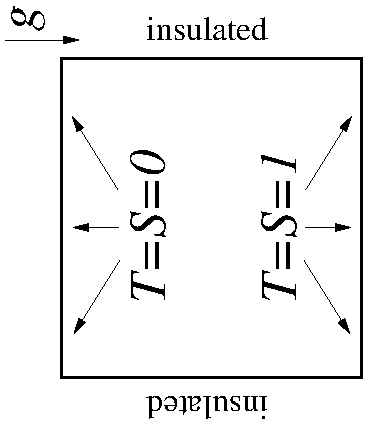
\includegraphics[width=.7\textwidth]{figures/setup}
  \end{center}
  \begin{center}
    \item $Ra := \frac{\rho^2 c_p \beta g \Delta T d^3}{k \mu}$
      \hspace{.5in} $Ma := \frac{ \rho c_p \dgammadT \Delta T d}{k \mu}$
      \hspace{.5in} $Pr := \frac{\mu c_p}{k}$
  \end{center}
\end{frame}




%%%%%%%%%%%%%%%%%%%%%%%%%%%%%%%%%%%%%%%%%%%%%%%%%%%%%%%%%%%%%%%%%%%%%%%%%%%%%%%
\subsection{Experiment vs. Simulation}
\begin{frame}
  \begin{itemize}
    
  \item Experiment 
    \begin{itemize}
    \item Disadvantages
      \begin{itemize}
      \item[$\circ$] Experimental uncertainty in $Ra$, $Ma$ sometimes 10-15\%.
      \item[$\circ$] Varying $d$ changes both $Ra$ and $Ma$, at different rates.
      \item[$\circ$] Complex laboratory setup
      \end{itemize}

    \item Advantages
      \begin{itemize}
      \item[$\circ$] A photo is worth a thousand words \ldots
      \end{itemize}
    \end{itemize}
 
  \item Simulation
    \begin{itemize}
    \item Disadvantages
      \begin{itemize}
      \item[$\circ$] Modeling errors
      \item[$\circ$] Computational resources
      \end{itemize}
   
    \item Advantages
      \begin{itemize}
      \item[$\circ$] May independently vary parameters
      \item[$\circ$] Can extract detailed information about the solution
      \end{itemize} 
    \end{itemize}
  \end{itemize}
\end{frame}



%%%%%%%%%%%%%%%%%%%%%%%%%%%%%%%%%%%%%%%%%%%%%%%%%%%%%%%%%%%%%%%%%%%%%%%%%%%%%%%
\subsection{Governing Equations}
\begin{frame}
  \only<1>
  {
    Incompressible Navier-Stokes with Boussinesq approximation:
    \begin{align}
      \nonumber
      \nabla \cdot \bv{u} &= 0
      \\
      \nonumber 
      \rho\left( \frac{\partial \bv{u}}{\partial t} + \bv{u}\cdot \nabla \bv{u} \right) &=
      \nabla \cdot \bv{\sigma} -\rho\beta\bv{g}(T-T_{ref}) 
      \\
      \nonumber
      \rho c_p \left(\frac{\partial T}{\partial t} + \bv{u}\cdot\nabla T\right) &=
      \nabla \cdot (k\nabla T)
    \end{align}

    \vspace{0.25in}

    With (Newtonian) stress tensor %$\bv{\sigma}$ is given by:
    \begin{equation*}
      \bv{\sigma} = -p \bv{I} + \mu \left(\nabla \bv{u} + \nabla \bv{u}^T \right)
    \end{equation*}
  }

  
  \only<2>
  {
    Incompressible Navier-Stokes -- Weak Statement:
    
    Find $\{\bv{u}, p, T\}$ satisfying
    \begin{align}
      % \nonumber
      \int_\Omega q \left( \nabla \cdot \bv{u}\right) d\Omega &= 0 
      \\
      \nonumber 
      \int_\Omega \left( \rho\left(
          \frac{\partial \bv{u}}{\partial t} + \bv{u} \cdot \nabla \bv{u}
	\right) \cdot \bv{v} + \bv{\sigma} : \nabla \bv{v} \right) d\Omega  &=
      \\ \nonumber
      - \int_\Omega \rho \beta \bv{g}(T-T_{ref})\cdot\bv{v} \; d\Omega&
      \\
      % \nonumber
      + \int_{\partial\Omega} \bv{\sigma}_n \cdot \bv{v} \; ds&
      \\
      % \nonumber
      \int_\Omega \left( \rho c_p \left(
          \frac{\partial T}{\partial t} + \bv{u} \cdot \nabla T
	\right) w + k \nabla T \cdot \nabla w \right) d\Omega &= 0
    \end{align}
    
    $\forall$ admissible $\bv{v}, q, w$.
  }
\end{frame}



%%%%%%%%%%%%%%%%%%%%%%%%%%%%%%%%%%%%%%%%%%%%%%%%%%%%%%%%%%%%%%%%%%%%%%%%%%%%%%%
\subsection{Boundary Conditions}
\begin{frame}
  \begin{itemize}
    \item The fluid velocity and temperature are subject to the following boundary conditions:
  \end{itemize}
  \vspace{.25in}
  \begin{center}
  \begin{tabular}{ccc} \toprule 
                         & Velocity & Temperature \\ \midrule
      Bottom Surface     & $\bv{u}$ = \mbox{\boldmath $0$}& $T = T_{h}$ \\ %\midrule
      Lateral Walls:     & $\bv{u}$ = \mbox{\boldmath $0$}& $\frac{\partial T}{\partial n} = 0$ \\ %\midrule
      Top (Free) Surface & \begin{tabular}{c}
                             $w = 0$ \\
                             $\frac{\partial u}{\partial z} = \dgammadT \frac{\partial T}{\partial x}$ \\
                             $\frac{\partial v}{\partial z} = \dgammadT \frac{\partial T}{\partial y}$
                           \end{tabular}
                         & \begin{tabular}{c}
                           \\
                           $\frac{\partial T}{\partial z} = \frac{\Delta T}{d}$
                           \\
                           \end{tabular} \\ \bottomrule
    \end{tabular}
  \end{center}
\end{frame}



%%%%%%%%%%%%%%%%%%%%%%%%%%%%%%%%%%%%%%%%%%%%%%%%%%%%%%%%%%%%%%%%%%%%%%%%%%%%%%%
\subsection{Numerical Method}
\begin{frame}
  \begin{itemize}
    \item 27-node tri-quadratic velocity, tri-linear pressure hexahedral elements % ($h^3$ accuracy)
    \item Standard Galerkin finite element formulation with Lagrangian basis
    \item ILU preconditioner and TFQMR linear solver via PETSc
    \item Crank-Nicolson time discretization %($\theta$ method with $\theta=1/2$)
    \item Fully coupled (solve for $\bv{u}, p, T$ simultaneously) implicit solution
    \item Dirichlet B.C.'s enforced via penalty %% modify only one matrix entry instead of all...
  \end{itemize}
\end{frame}



%%%%%%%%%%%%%%%%%%%%%%%%%%%%%%%%%%%%%%%%%%%%%%%%%%%%%%%
\subsection{Computational Challenges}
\begin{frame}
  \begin{itemize}
    \item Time accurate, fully coupled simulations are expensive
    \item Need to use parallel machines to solve large-scale problems
    \item High-quality domain decomposition crucial for scalability
    \item Lack of commercial software to meet these needs
  \end{itemize}
\end{frame}



%%%%%%%%%%%%%%%%%%%%%%%%%%%%%%%%%%%%%%%%%%%%%%%%%%%%%%%
\subsection{Domain Decomposition}
\begin{frame}
    \only<1>
    {
      \setlength{\parindent}{0pt}
      % \zerolistvertdimens
      \begin{minipage}[h]{.7\textwidth}
	\begin{figure}[h]
	  \centering
            % This figure has been lost
            % \includegraphics[width=.8\textwidth]{figures/streamtraces}
	\end{figure}
      \end{minipage}
      \begin{minipage}[h]{.3\textwidth}
	\small
	\raggedright
	\begin{itemize}
	  
 	  \item $Ra=10^5$
	  \item No-slip surfaces,  \\ $T=307-7 x/w$
	  \item Simulated for 30 seconds
	\end{itemize}
	\normalsize	
      \end{minipage}
    }

    \only<2>
    {
      \begin{minipage}[h]{.45\textwidth}
	\begin{figure}[h]
	  \centering
            \includegraphics[width=\textwidth]{figures/part_trans}
	\end{figure}
      \end{minipage}
      % 
      \begin{minipage}[h]{.45\textwidth}
	\begin{figure}[h]
	  \centering
            \includegraphics[width=\textwidth]{figures/part_exp_trans}
	\end{figure}
      \end{minipage}
    }
\end{frame}




%%%%%%%%%%%%%%%%%%%%%%%%%%%%%%%%%%%%%%%%%%%%%%%%%%%%%%%%%%%%%%%%%%%%%%%%%%%%%%%
\subsection{Results}
\begin{frame}
  \begin{center}
  \begin{tabular}{ccc} \\
    \textbf{4 cells} &
    % \href{movies/4cell.avi}
    \includegraphics[width=.3\textwidth]{figures/4cell} &
    \includegraphics[width=.3\textwidth]{figures/4cell_max_w} \\
  \end{tabular}
 \begin{tabular}{ccc} \\
   \textbf{5 cells} &
   %\href{movies/5cell.avi}
   \includegraphics[width=.3\textwidth]{figures/5cell} &
   \includegraphics[width=.3\textwidth]{figures/5cell_max_w} \\
 \end{tabular}
  \end{center}
\end{frame}





%%%%%%%%%%%%%%%%%%%%%%%%%%%%%%%%%%%%%%%%%%%%%%%%%%%%%%%%%%%%%%%%%%%%%%%%%%%%%%%
\begin{frame}
  \tiny
  \begin{tabular}{ccccc} \\
    
    %% 1 and 4 cell configurations
    \includegraphics[width=.2\textwidth]{figures/1cell_exp} &
    \includegraphics[width=.2\textwidth]{figures/1cell_AR3} &
    \hspace{.05\textwidth} &
    \includegraphics[width=.2\textwidth]{figures/4cell_exp} &
    \includegraphics[width=.2\textwidth]{figures/4cell_AR6point5} \\
    
    $228$ / $380$ / $1.82$ &
    $30$  / $92$  / $3.0$ &
    & %gap
    $38$ / $93$ / $6.36$ &
    $30$  / $92$  / $6.5$ \\

    %% 2 and 5 cell configurations
    \includegraphics[width=.2\textwidth]{figures/2cell_exp} &
    \includegraphics[width=.2\textwidth]{figures/2cell_AR5point5} &
    \hspace{.05\textwidth} &
    \includegraphics[width=.2\textwidth]{figures/5cell_exp} &
    \includegraphics[width=.2\textwidth]{figures/5cell_AR8} \\

    $33$  / $64$  / $5.68$ &
    $30$  / $92$  / $5.5$ &
    & %gap
    $19$  / $80$  / $8.08$ &
    $30$  / $92$  / $8$ \\
    
    %% 3 and 6 cell configurations
    \includegraphics[width=.2\textwidth]{figures/3cell_exp} &
    \includegraphics[width=.2\textwidth]{figures/3cell_AR6} &
    \hspace{.05\textwidth} &
    \includegraphics[width=.2\textwidth]{figures/6cell_exp} &
    \includegraphics[width=.2\textwidth]{figures/6cell_AR8point4} \\

    $42$  / $96$  / $6.18$ &
    $30$  / $92$  / $6$ &
    & %gap
    $22$  / $86$  / $8.08$ &
    $30$  / $92$  / $8.2$ \\ % This should really be 8.4
    
  \end{tabular}
  
  % \centerline{ Non-dimensional parameters for \emph{all} numerical simulations: $Ma=92$, $Ra=30$}
  \centerline{$Ra$ / $Ma$ / $\Gamma$ }

\end{frame}





%%%%%%%%%%%%%%%%%%%%%%%%%%%%%%%%%%%%%%%%%%%%%%%%%%%%%%%%%%%%%%%%%%%%%%%%%%%%%%%
% Not necessary with Darmstadt
% \begin{frame}
%   \tableofcontents[currentsection,hideallsubsections]
% \end{frame}


\section{Elder Problem}

%%%%%%%%%%%%%%%%%%%%%%%%%%%%%%%%%%%%%%%%%%%%%%%%%%%%%%%%%%%%%%%%%%%%%%%%%%%%%%%
\subsection{Problem Description}
\begin{frame}
  \centerline{\includegraphics[width=\textwidth]{figures/elder}}
\end{frame}




%%%%%%%%%%%%%%%%%%%%%%%%%%%%%%%%%%%%%%%%%%%%%%%%%%%%%%%%%%%%%%%%%%%%%%%%%%%%%%%
\subsection{Governing Equations}
\begin{frame}
  Equations governing transport of species $c$ in a porous medium:
  \begin{eqnarray}
    \nonumber
    \varepsilon \frac{\partial \rho}{\partial c}\frac{\partial c}{\partial t} + \nabla \cdot
    \left( \rho \bv{v} \right) &=&0 \\
    \nonumber
    \varepsilon \rho \frac{\partial c}{\partial t} + \rho \bv{v} \cdot \nabla c
    - \nabla \cdot \left( \varepsilon \rho D \nabla c
    \right) &=&0 
  \end{eqnarray}

%%   Closed with Darcy's law relating velocity to the pressure gradient:
%%   \begin{equation}
%%     \label{eqn:porous_Darcy}
%%     \nonumber
%%     \bv{v} = - \frac{\bv{k}}{\mu} \left( \nabla{p} - \rho \bv{g} \right)
%%   \end{equation}

  \small
  Observations
  \begin{itemize}
    
    \item Forms a transient, nonlinear $\left(\rho = \rho\left(c\right)\right)$ coupled set of equations.
    \item Sensitive to initial conditions.
  \end{itemize}
  \normalsize
\end{frame}



%%%%%%%%%%%%%%%%%%%%%%%%%%%%%%%%%%%%%%%%%%%%%%%%%%%%%%%%%%%%%%%%%%%%%%%%%%%%%%%
\begin{frame}
    \begin{itemize}
    \item The governing equations describe the transport of a species concentration $c$
      in a porous medium of density $\rho$.
    \item Important applications in nuclear waste disposal and groundwater pollution
      impact predictions.
    \item Usually employ \emph{Darcy's Law} to relate the flow velocity
      to the pressure in the medium:
      \begin{equation}
	\bv{v} = - \frac{\bv{K}}{\mu} \left( \nabla p - \rho \bv{g}
	\right)
	\nonumber
      \end{equation}
    \item Characterized by complicated material properties in the
      porous medium $(\epsilon, D)$ and nonlinearities in the density-concentration coupling
  \end{itemize}
\end{frame}



%%%%%%%%%%%%%%%%%%%%%%%%%%%%%%%%%%%%%%%%%%%%%%%%%%%%%%%%%%%%%%%%%%%%%%%%%%%%%%%
\subsection{Results}
\begin{frame}
  \centerline{\includegraphics[angle=270,width=\textwidth]{figures/elder_amr}}
  % Note: movies weren't playing on my Mac
  %\footnotesize
  %\href{movies/elder_soln.avi}{solution},
  %\href{movies/elder_mesh.avi}{mesh}
  %\normalsize
\end{frame}




\section{E. coli}


%%%%%%%%%%%%%%%%%%%%%%%%%%%%%%%%%%%%%%%%%%%%%%%%%%%%%%%%%%%%%%%%%%%%%%%%%%%%%%%
% Not necessary with Darmstadt
% \begin{frame}
%   \tableofcontents[currentsection,hideallsubsections]
% \end{frame}




%%%%%%%%%%%%%%%%%%%%%%%%%%%%%%%%%%%%%%%%%%%%%%%%%%%%%%%%%%%%%%%%%%%%%%%%%%%%%%%
\subsection{Problem Description}
\begin{frame}
  \begin{itemize}
    
    \item Experimentalists observe complex pattern formation in \emph{E. coli} specimens.
    \item These patterns only occur in the presence of \emph{chemotaxis}.
    \item When chemotaxis is sufficiently strong compared to diffusion, complex patterns may develop.
    \item Understanding the relationship between pattern formation and system parameters
          enables interesting applications:
    \begin{itemize}
      \item System diagnosis.
      \item Detection of atmospheric pollutants.
    \end{itemize}
  \end{itemize}
\end{frame}



%%%%%%%%%%%%%%%%%%%%%%%%%%%%%%%%%%%%%%%%%%%%%%%%%%%%%%%%%%%%%%%%%%%%%%%%%%%%%%%
\subsection{Governing Equations}
\begin{frame}
  \begin{align}
    \frac{\partial u}{\partial t} & = d_u \Delta u - \alpha \nabla \cdot \left[ \frac{u}{(1+ v)^2} \nabla v \right]
                                      + \rho u \left( \delta \frac{w^2}{1 + w^2} - u \right) \nonumber \\
    \frac{\partial v}{\partial t} & = \;\;\;\; \Delta v + \beta w \frac{u^2}{\mu + u^2} - uv \nonumber \\
    \frac{\partial w}{\partial t} & = d_w \Delta w - \kappa u \frac{w^2}{1 + w^2} \nonumber
  \end{align}
  where $u,v,w$ are the concentration of \emph{E. coli}, chemoattractant, and food source, respectively.
\end{frame}




%%%%%%%%%%%%%%%%%%%%%%%%%%%%%%%%%%%%%%%%%%%%%%%%%%%%%%%%%%%%%%%%%%%%%%%%%%%%%%%
\subsection{Results}
\begin{frame}
    \only<1>
    {
      \begin{center}
	\begin{tabular}{cc}
	  \includegraphics[height=.4\textheight]{figures/ecoli0010} &
	  \includegraphics[height=.4\textheight]{figures/ecoli0015} \\ 
	  \includegraphics[height=.4\textheight]{figures/ecoli0022} &
	  \includegraphics[height=.4\textheight]{figures/ecoli0028} \\
	\end{tabular}
      \end{center}
      \footnotesize
      \href{movies/plate_pattern_3.avi}{experiment}
    }
    \only<2>
    {
      \begin{center}
	\begin{tabular}{cc}
	  \includegraphics[height=.4\textheight]{figures/mesh0010} &
	  \includegraphics[height=.4\textheight]{figures/mesh0015} \\ 
	  \includegraphics[height=.4\textheight]{figures/mesh0022} &
	  \includegraphics[height=.4\textheight]{figures/mesh0028} \\
	\end{tabular}
      \end{center}
      \footnotesize
      \href{movies/plate_pattern_3.avi}{experiment}
    }
\end{frame}



\section{Hardware}

%%%%%%%%%%%%%%%%%%%%%%%%%%%%%%%%%%%%%%%%%%%%%%%%%%%%%%%%%%%%%%%%%%%%%%%%%%%%%%%
% Not necessary with Darmstadt
% \begin{frame}
%   \tableofcontents[currentsection,hideallsubsections]
% \end{frame}


%%%%%%%%%%%%%%%%%%%%%%%%%%%%%%%%%%%%%%%%%%%%%%%%%%%%%%%%%%%%%%%%%%%%%%%%%%%%%%%
\begin{frame}%{Hardware}
  \only<1-2>
  {
    \begin{columns}
      \column{.5\textwidth}
      CFDLab cluster: ``\emph{bbrox}''
      \begin{itemize}
      \item 17 Intel C440GX+ boards with dual Pentium~III 550MHz processors
      \item 32 550MHz processors
      \item 18 GB RAM
      \item 134 GB disk
      \end{itemize}

      \column{.4\textwidth}
      \only<1> { \centerline{\includegraphics[height=.8\textheight]{figures/bbrox_front}} }
      \only<2> { \centerline{\includegraphics[height=.8\textheight]{figures/bbrox_back}} }
    \end{columns}
  }
  \only<3>
  {
    \begin{columns}
      \column{.5\textwidth}
      
      Texas Advanced Computing Center (TACC) cluster: ``\emph{longhorn}''
      
      \begin{itemize}
      \item IBM Power4 System composed of p690 and p655 nodes
      \item 224 1GHz processors
      \item 512 GB RAM
      \item 7.1 TB disk
      \end{itemize}

      \column{.4\textwidth}
      \centerline{\includegraphics[width=\textwidth]{figures/p690_door}}
    \end{columns}
  }
  \only<4-5>
  {
    \begin{columns}
      \column{.4\textwidth}
      TACC cluster: ``\emph{lonestar}''
      \begin{itemize}
      \item Cray-Dell Cluster
      \item 600 3GHz processors
      \item 600 GB RAM
      \item 15 TB disk
      \end{itemize}

      \column{.5\textwidth}
      \only<4> { \centerline{\includegraphics[width=\textwidth]{figures/lonestar}}  }
      \only<5> { \centerline{\includegraphics[width=\textwidth]{figures/lonestar2}} }
    \end{columns}
  }
\end{frame}
 


\section{Software}

%%%%%%%%%%%%%%%%%%%%%%%%%%%%%%%%%%%%%%%%%%%%%%%%%%%%%%%%%%%%%%%%%%%%%%%%%%%%%%%
% Not necessary with Darmstadt
% \begin{frame}
%   \tableofcontents[currentsection,hideallsubsections]
% \end{frame}

 
%%%%%%%%%%%%%%%%%%%%%%%%%%%%%%%%%%%%%%%%%%%%%%%%%%%%%%%%%%%%%%%%%%%%%%%%%%%%%%%
\subsection{MPI}
\begin{frame}%{MPI}
  Scenario: Input data file lives on a network file system.  What
  is the best way to get the input onto all the processors?
  \begin{itemize} 
    \item Solution 1: (na\"{i}ve implementation) Have all processors simultaneously
      read the file over the network.  This solution is not scalable, and generates
      considerable network traffic.
    \item Solution 2: Have a designated processor read the input file, then use \texttt{MPI\_Bcast}
      to broadcast the data to the remaining processors. Network traffic is reduced, and
      algorithmic complexity is $\mathcal{O}(\log_2 n_\text{proc})$.
  \end{itemize}
\end{frame}



%%%%%%%%%%%%%%%%%%%%%%%%%%%%%%%%%%%%%%%%%%%%%%%%%%%%%%%%%%%%%%%%%%%%%%%%%%%%%%%
\begin{frame}%{MPI}
  \begin{itemize}
    \item 8 Processor Broadcast
    \begin{itemize}
      \item Data on processor 0
      \item All processors need information
    \end{itemize}
  %\item 3 Steps ($O(\log_2 n_\text{proc})$)
  \end{itemize}

  \only<1>
  {
    \begin{minipage}{.2\textwidth}
      Beginning
    \end{minipage}
    \begin{minipage}{.8\textwidth}
      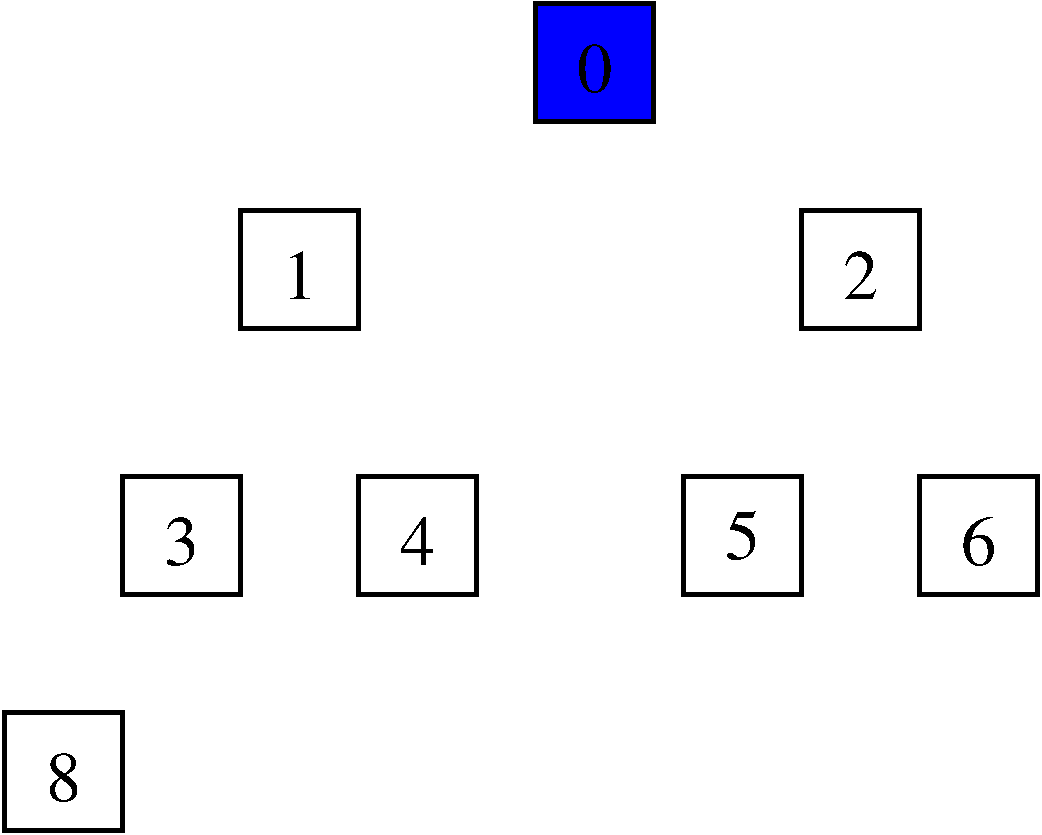
\includegraphics[width=.7\textwidth]{figures/bcast-1}
    \end{minipage}
  }
  \only<2>
  {
    \begin{minipage}{.2\textwidth}
      Step 1
    \end{minipage}
    \begin{minipage}{.8\textwidth}
      \includegraphics[width=.7\textwidth]{figures/bcast0}
    \end{minipage}
  }
  \only<3>
  {
    \begin{minipage}{.2\textwidth}
      Step 2
    \end{minipage}
    \begin{minipage}{.8\textwidth}
      \includegraphics[width=.7\textwidth]{figures/bcast1}
    \end{minipage}
  }
  \only<4>
  {
    \begin{minipage}{.2\textwidth}
      Step 3
    \end{minipage}
    \begin{minipage}{.8\textwidth}
      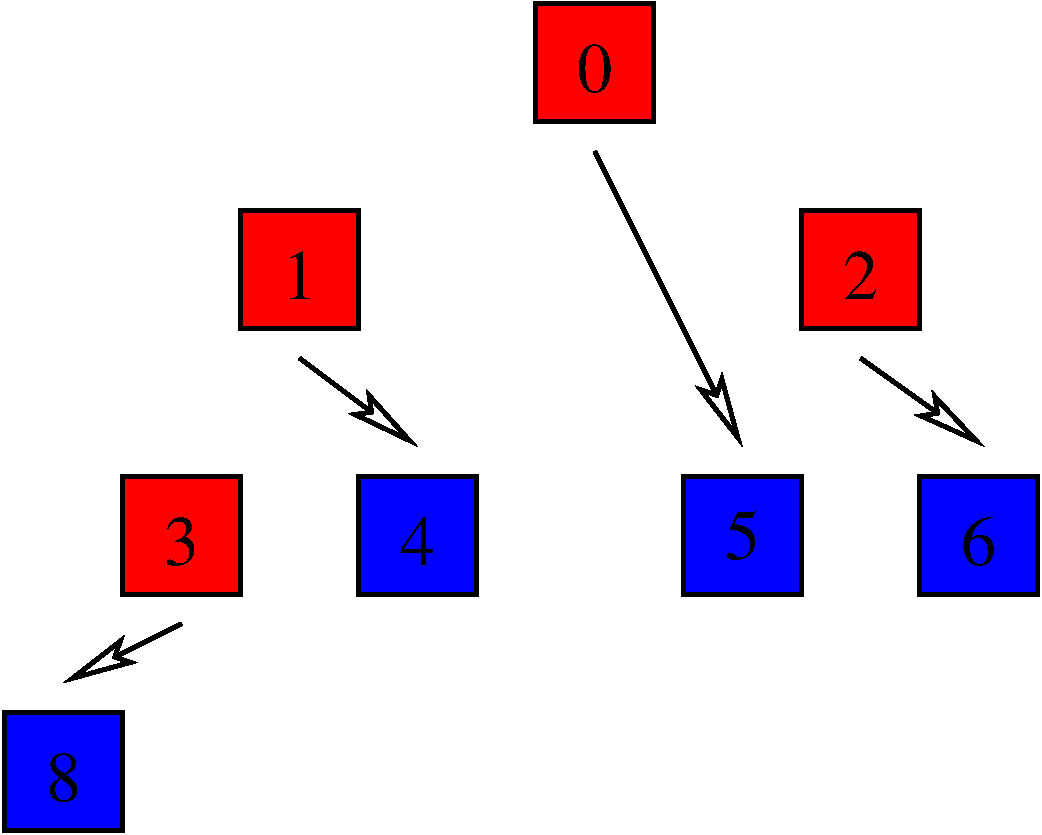
\includegraphics[width=.7\textwidth]{figures/bcast2}
    \end{minipage}
  }
\end{frame}


%%%%%%%%%%%%%%%%%%%%%%%%%%%%%%%%%%%%%%%%%%%%%%%%%%%%%%%%%%%%%%%%%%%%%%%%%%%%%%%
\begin{frame}%{MPI}
  \begin{itemize}
    \item Broadcast performance over 10/100 Ethernet and Myrinet vs.\ message size
  \end{itemize}
  \begin{center}
    \includegraphics[width=.7\textwidth]{figures/perf_broadcast}
  \end{center}
\end{frame}


%%%%%%%%%%%%%%%%%%%%%%%%%%%%%%%%%%%%%%%%%%%%%%%%%%%%%%%%%%%%%%%%%%%%%%%%%%%%%%%
\subsection{METIS}
\begin{frame}%{METIS}
  \begin{itemize}
    \item \href{http://www-users.cs.umn.edu/~karypis/metis/}{METIS} provides graph partitioning and sparse matrix ordering algorithms
    \item Provides several key components:
      \begin{itemize}
        \item Static graph partitioning
        \item Static mesh partitioning
        \item Fill-reducing reordering
      \end{itemize}
    \item \href{http://www-users.cs.umn.edu/~karypis/metis/}{ParMETIS} works in parallel and also provides dynamic graph partitioning
  \end{itemize}
\end{frame}


%%%%%%%%%%%%%%%%%%%%%%%%%%%%%%%%%%%%%%%%%%%%%%%%%%%%%%%%%%%%%%%%%%%%%%%%%%%%%%%
\begin{frame}%{METIS}
  \centerline{\includegraphics[height=.88\textheight]{figures/ML-Idea}}
\end{frame}


%%%%%%%%%%%%%%%%%%%%%%%%%%%%%%%%%%%%%%%%%%%%%%%%%%%%%%%%%%%%%%%%%%%%%%%%%%%%%%%
\begin{frame}%{METIS}
  \only<1> {\centerline{\includegraphics[height=.8\textheight]{figures/geometry_transparent}}}
  \only<2> {\centerline{\includegraphics[height=.8\textheight]{figures/part_trans}}}
\end{frame}


%%%%%%%%%%%%%%%%%%%%%%%%%%%%%%%%%%%%%%%%%%%%%%%%%%%%%%%%%%%%%%%%%%%%%%%%%%%%%%%
\subsection{libMesh}
\begin{frame}%{libMesh}
  \begin{itemize} % [\texttt{http://libmesh.sourceforge.net}]
    \item \texttt{libMesh}: Finite-element library developed by Kirk, Peterson, et.~al.\
       at the University of Texas at Austin with international collaboration.
      \begin{itemize}
        \item C++ class library using the Standard Template Library
        \item Interface to PETSc and LASPACK linear solvers
        \item Interface to ParMETIS partitioning library
        \item Unstructured hybrid 2D and 3D meshes
        \item Lagrange, Hierarchic, Szabab, and Discontinuous finite elements
        \item Runs on many platforms with \emph{native} compilers
	\item Supports real or complex variables
        \item Adaptive $h$-refinement
	\item Open Source: \url{http://libmesh.sourceforge.net}
      \end{itemize}
  \end{itemize}
\end{frame}


%%%%%%%%%%%%%%%%%%%%%%%%%%%%%%%%%%%%%%%%%%%%%%%%%%%%%%%%%%%%%%%%%%%%%%%%%%%%%%%
\subsection{MGF}
\begin{frame}[fragile]
\begin{itemize}
  \item Finite element code developed by R.~McLay and B.~Barth at the University of Texas
        CFDLab under a NASA Grand Challenge Grant
  \item Used to successfully solve problems in
        porous media transport, non-Newtonian fluid flow, chemical reaction-diffusion,
        and some biological applications
  \item Physics models in the form of partial differential equations
        can be integrated directly into \texttt{MGF}
\end{itemize}

\vspace{-.075\textheight}
\begin{columns}
  
\column{.55\textwidth}

\small
\begin{semiverbatim}
\\begin\{equation\}
  \\eqnVar\{T\}
  \\label\{eq:thermal\}
  \\int \\rho*c\_p*\\phi*\\pdv\{T\}\{t\}
  + \\rho*c\_p*v*\\grad\{T\}*\\phi 
  + k*\\grad\{\\phi\}*\\grad\{T\} \\dx
  = \\int Q*\\phi \\dx
\\end\{equation\}
\end{semiverbatim}
\normalsize

\column{.005\textwidth}

$\Leftrightarrow$

\column{.4\textwidth}

\scriptsize
\begin{align}
  \nonumber
  \int \rho c_p \frac{\partial T}{\partial t} \phi \;dx & + \mbox{}
  \\
  \nonumber
  \int \rho c_p \bv{v} \cdot \nabla T \phi \;dx & + \mbox{}
  \\
  \nonumber
  \int k \nabla T \cdot \nabla \phi \;dx &=
  \\
  \nonumber
  \int Q \phi \;dx
\end{align}
\normalsize


\end{columns}

\end{frame}



%%%%%%%%%%%%%%%%%%%%%%%%%%%%%%%%%%%%%%%%%%%%%%%%%%%%%%%%%%%%%%%%%%%%%%%%%%%%%%%
%\subsection{Solver Scalability}
\begin{frame}
  \begin{itemize}
  \item Solver Scalability
  \end{itemize}
    \only<1>{
      \begin{minipage}{.5\textwidth}
	\centering
	\includegraphics[width=\textwidth]{figures/scale2}
      \end{minipage}
      \hspace{.02\textwidth}
      \begin{minipage}{.4\textwidth}
	\raggedright
	\begin{itemize}
	\item EBE Bi-CGStab
	\item BLAS for MATVECs, dot products, etc.
	\item Memory bandwidth limited
	  % \item 7\% of theoretical peak (on the P4)
	\end{itemize}
      \end{minipage}
    }
    \only<2>{
      \begin{minipage}{.5\textwidth}
	\centering
	\includegraphics[width=\textwidth]{figures/scale1}
      \end{minipage}
      \hspace{.02\textwidth}
      \begin{minipage}{.4\textwidth}
	\raggedright
	\begin{itemize}
	\item EBE Bi-CGStab
	\item BLAS for MATVECs, dot products, etc.
	\item Memory bandwidth limited
	  % \item 7\% of theoretical peak (on the P4)
	\end{itemize}
      \end{minipage}
    }
\end{frame}



%%%%%%%%%%%%%%%%%%%%%%%%%%%%%%%%%%%%%%%%%%%%%%%%%%%%%%%%%%%%%%%%%%%%%%%
\begin{frame}%{SMP: Less is more?}

\begin{itemize}

%\item Results are for the MGF code developed in the CFDLab
%\item Different applications stress machines in different ways
\item In general, sparse linear algebra allows little cache reuse
  \begin{itemize}
  \item Generally limited by \emph{memory bandwidth}
  \item SMP nodes offer little performance benefit
  \end{itemize}
\item For memory-bandwidth bound applications single processor nodes will give better speedup
\item This is changing with AMD Opteron and recent P4's
\end{itemize}

\tiny
%%   \begin{tabular}{|c|r|r||r|r|r||r|r||r|r||r||r|r|r|} \hline
%%     & \multicolumn{2}{|c||}{\textbf{Pentium II}} & \multicolumn{3}{|c||}{\textbf{Pentium III}} &
%%     \multicolumn{2}{|c||}{\textbf{PII Xeon}} &
%%     \multicolumn{2}{|c||}{\textbf{PIII Xeon}} &
%%     \multicolumn{1}{|c||}{\textbf{Alpha}} &
%%     \multicolumn{2}{|c|}{\textbf{P4 Xeon}} \\ \hline 
%%     \textbf{Chip (MHz)}    & 266  & 350  & 550   & 850   & 850x2 & 400  & 400x2 & 550   & 550x2 & 500   & 1700  & 1700x2  \\ \hline
%% %% Overall (MFlops) & 43   & 75   & 97    & 115   & 123   & 80   & 129   & 103   & 117   & 93    & 309   & 501     \\ \hline
%% %% 1 Proc Solve     & 42.2 & 75.3 & 96.4  & 110.2 & 57.0  & 81.7 & 62.4  & 101.6 & 58.8  & 95.2  & 307.2 & 251.8   \\ \hline
%% %% 1 Proc FKF       & 55.2 & 71.3 & 100.7 & 182.5 & 180.1 & 68.7 & 86.4  & 114.5 & 58.7  & 80.0  & 377.0 & 216.5   \\ \hline
%%     \begin{minipage}{1.1in}
%%       \begin{center}
%% 	\textbf{MatVec} \\ 
%% 	\textbf{(MFlops)}
%%       \end{center}
%%       \end{minipage} & 43.9 & 79.9 & 100.0 & 114.7 & 119.2 & 84.2 & 129.8  & 106.0 & 121.4  & 100.4 & 311.3 & 533.4   \\ \hline
%%   \end{tabular}    
%%  \hspace{-.5in}

  \begin{tabular}{crrrrrc} \toprule
    & \multicolumn{2}{c}{\textbf{Pentium II}}
    & \multicolumn{3}{c}{\textbf{Pentium III}}
    & \multicolumn{1}{c}{
      \begin{minipage}{1.2in}
	\begin{center}
	\textbf{Pentium 4 \\(800MHz FSB)}
	\end{center}
    \end{minipage}}
    \\ \midrule 
    \textbf{Chip (MHz)}    & 266  & 350  & 550   & 850   & 850x2 & 3000 \\ \midrule
	\textbf{MatVec} \\ 
	\textbf{(MFlop/s)}
        & 43.9 & 79.9 & 100.0 & 114.7 & 119.2 & 595   \\ \midrule
    \textbf{MFlop/s per MHz} & 0.165 & 0.228 & 0.1818 & 0.1349 & (n/a) & 0.1983\\ \bottomrule
  \end{tabular}

\begin{center}
\begin{tabular}{crrrrrr} \toprule
    & \multicolumn{2}{c}{\textbf{PII Xeon}} &
    \multicolumn{2}{c}{\textbf{PIII Xeon}} &
    \multicolumn{2}{c}{\textbf{P4 Xeon}} \\ \midrule 
    \textbf{Chip (MHz)}    & 400  & 400x2 & 550   & 550x2 & 1700  & 1700x2  \\ \midrule
%% Overall (MFlops) & 43   & 75   & 97    & 115   & 123   & 80   & 129   & 103   & 117   & 93    & 309   & 501     \\ \hline
%% 1 Proc Solve     & 42.2 & 75.3 & 96.4  & 110.2 & 57.0  & 81.7 & 62.4  & 101.6 & 58.8  & 95.2  & 307.2 & 251.8   \\ \hline
%% 1 Proc FKF       & 55.2 & 71.3 & 100.7 & 182.5 & 180.1 & 68.7 & 86.4  & 114.5 & 58.7  & 80.0  & 377.0 & 216.5   \\ \hline
%    \begin{minipage}{1.1in}
%      \begin{center}
	\textbf{MatVec} \\ 
	\textbf{(MFlop/s)}
%      \end{center}
%      \end{minipage} 
        & 84.2 & 129.8  & 106.0 & 121.4  & 311.3 & 533.4   \\ \midrule
    \textbf{MFlop/s per MHz} & 0.2105 & (n/a) & 0.1927 & (n/a) & 0.1831 & (n/a) \\ \bottomrule
  \end{tabular}
\end{center}
\normalsize


\end{frame}




%%%%%%%%%%%%%%%%%%%%%%%%%%%%%%%%%%%%%%%%%%%%%%%%%%%%%%%%%%%%%%%%%%%%%%%%%%%%%%%
% \begin{frame}{Other Containers}
%   % This image has been lost some time in the intervening years... :(
%   % \centerline{\href{movies/triangle_hi_res.avi}{\includegraphics[width=.9\textwidth]{figures/triangle_contours}}}
% \end{frame}





\section{Conclusion}

%%%%%%%%%%%%%%%%%%%%%%%%%%%%%%%%%%%%%%%%%%%%%%%%%%%%%%%%%%%%%%%%%%%%%%%%%%%%%%%
\subsection{Conclusions}
\begin{frame}%{Conclusions}
  \begin{itemize}
    
    \item The finite element method is broadly applicable to general PDEs.  \emph{Not just structures!}
      \begin{itemize}
	\item Fluid flows
	\item Biological applications
      \end{itemize}
    \item Current research areas include:
      \begin{itemize}
	\item Efficient parallel adaptive finite element methods
	\item \emph{a posteriori} error estimation
	\item Sensitivities in nonlinear PDEs
	\item Software frameworks for large-scale multiphysics applications
      \end{itemize}
  \end{itemize}
\end{frame}



%%%%%%%%%%%%%%%%%%%%%%%%%%%%%%%%%%%%%%%%%%%%%%%%%%%%%%%%%%%%%%%%%%%%%%%%%%%%%%%
\subsection{Acknowledgements}
\begin{frame}%{Acknowledgements}
  I would like to thank:

  \begin{itemize}
    \item Dr. Graham Carey \& Bill Barth for many useful discussions
    \item The U.S. Department of Energy for sponsoring much of this work
  \end{itemize}
\end{frame}



%%%%%%%%%%%%%%%%%%%%%%%%%%%%%%%%%%%%%%%%%%%%%%%%%%%%%%%%%%%%%%%%%%%%%%%%%%%%%%%
\subsection{Questions?}
\begin{frame}%{Questions?}
  \centerline{\includegraphics[height=.8\textheight]{figures/smiley2}}
\end{frame}








\end{document}


%% Local Variables:
%% mode: latex
%% End:
 
% LocalWords:  PDEs discretization Galerkin Linearization Jacobian ds
% LocalWords:  BCG GMRES TOL Marangoni tourbillons cellulaires dans
% LocalWords:  une nappe liquide Incompressible Navier Boussinesq ccc
% LocalWords:  tri hexahedral ILU preconditioner TFQMR PETSc Nicolson
% LocalWords:  scalability ccccc nonlinearities coli Experimentalists
% LocalWords:  chemotaxis uv chemoattractant CFDLab bbrox GX TACC MPI
% LocalWords:  lonestar na ve scalable Bcast proc Myrinet METIS et al
% LocalWords:  ParMETIS libMesh LASPACK Szabab MGF McLay eqnVar eq dx
% LocalWords:  pdv EBE CGStab BLAS MATVECs SMP AMD Opteron crrrrrc
% LocalWords:  FSB MatVec MFlop crrrrrr PII Xeon PIII posteriori
% LocalWords:  multiphysics Acknowledgements
